\begin{figure}[t]
  \centering
  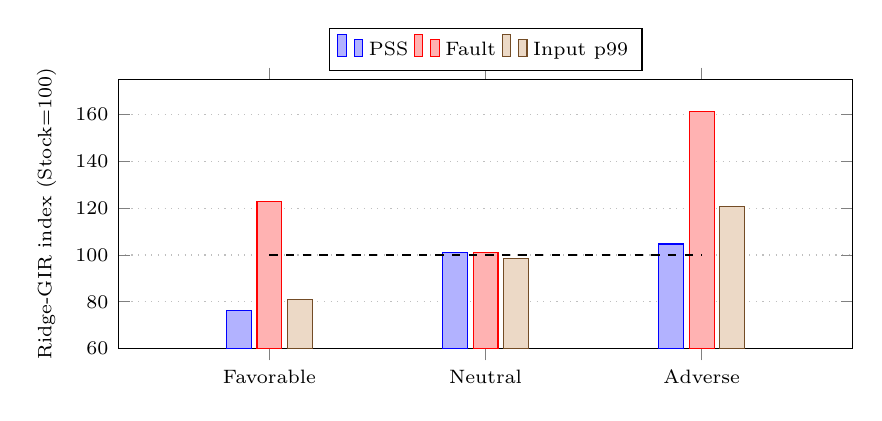
\begin{tikzpicture}
  \begin{axis}[
    width=0.9\linewidth, height=5.0cm, ybar=2pt, bar width=9pt,
    ymin=60, ymax=175, symbolic x coords={Favorable,Neutral,Adverse}, xtick=data,
    ylabel={Ridge-GIR index (Stock${=}100$)}, ylabel style={font=\scriptsize},
    tick label style={font=\scriptsize}, ytick={60,80,100,120,140,160},
    legend style={font=\scriptsize, at={(0.5,1.03)}, anchor=south, legend columns=3},
    enlarge x limits=0.35, ymajorgrids, major grid style={dotted}]
  \addplot coordinates {(Favorable,76.1) (Neutral,100.9) (Adverse,104.7)};
  \addplot coordinates {(Favorable,122.7) (Neutral,101.2) (Adverse,161.2)};
  \addplot coordinates {(Favorable,81.0) (Neutral,98.6) (Adverse,120.6)};
  \draw[dashed] (axis cs:Favorable,100) -- (axis cs:Adverse,100);
  \legend{PSS, Fault, Input p99}
  \end{axis}
  \end{tikzpicture}
  \caption{Cross-regime robustness of the coordinated learned policy
  ($\textsf{Ridge-GIR}$). Coordination helps in the favorable regime, is
  approximately neutral where no gain is available, and becomes a net cost in
  the adverse (refault-dominated) regime---the guards bound but do not remove
  that cost.}
  \label{fig:regimes}
\end{figure}
